\documentclass{article}
\usepackage{scribe}
\usepackage{amssymb}
\usepackage{amsmath}

\newtheorem{hw}{Homework Problem}
\newtheorem{ex}{Example}

\newcommand{\Perp}{{\bot\negthickspace\negthickspace\bot}}


%%% Unless you have very specific needs, the lines above should include
%%% all the typesetting features you need.

 


\begin{document}

\begin{lecture}{September 4th, 2004}{Yongyi Mao}



\section{Opening}

The reason we are here is to learn deep learning, because

\begin{enumerate}
\item Deep learning is cool
\item Deep learning is useful
\end{enumerate} 

The logo of the course is shown in Figure \ref{fig:logo}. The course requires some math and lots of programming. The framework you need to use can be either one of the following two:

\begin{enumerate}
\item TensorFlow
\item Pytorch
\end{enumerate} 

\begin{figure}[ht!]
\centering
\scalebox{0.15}{
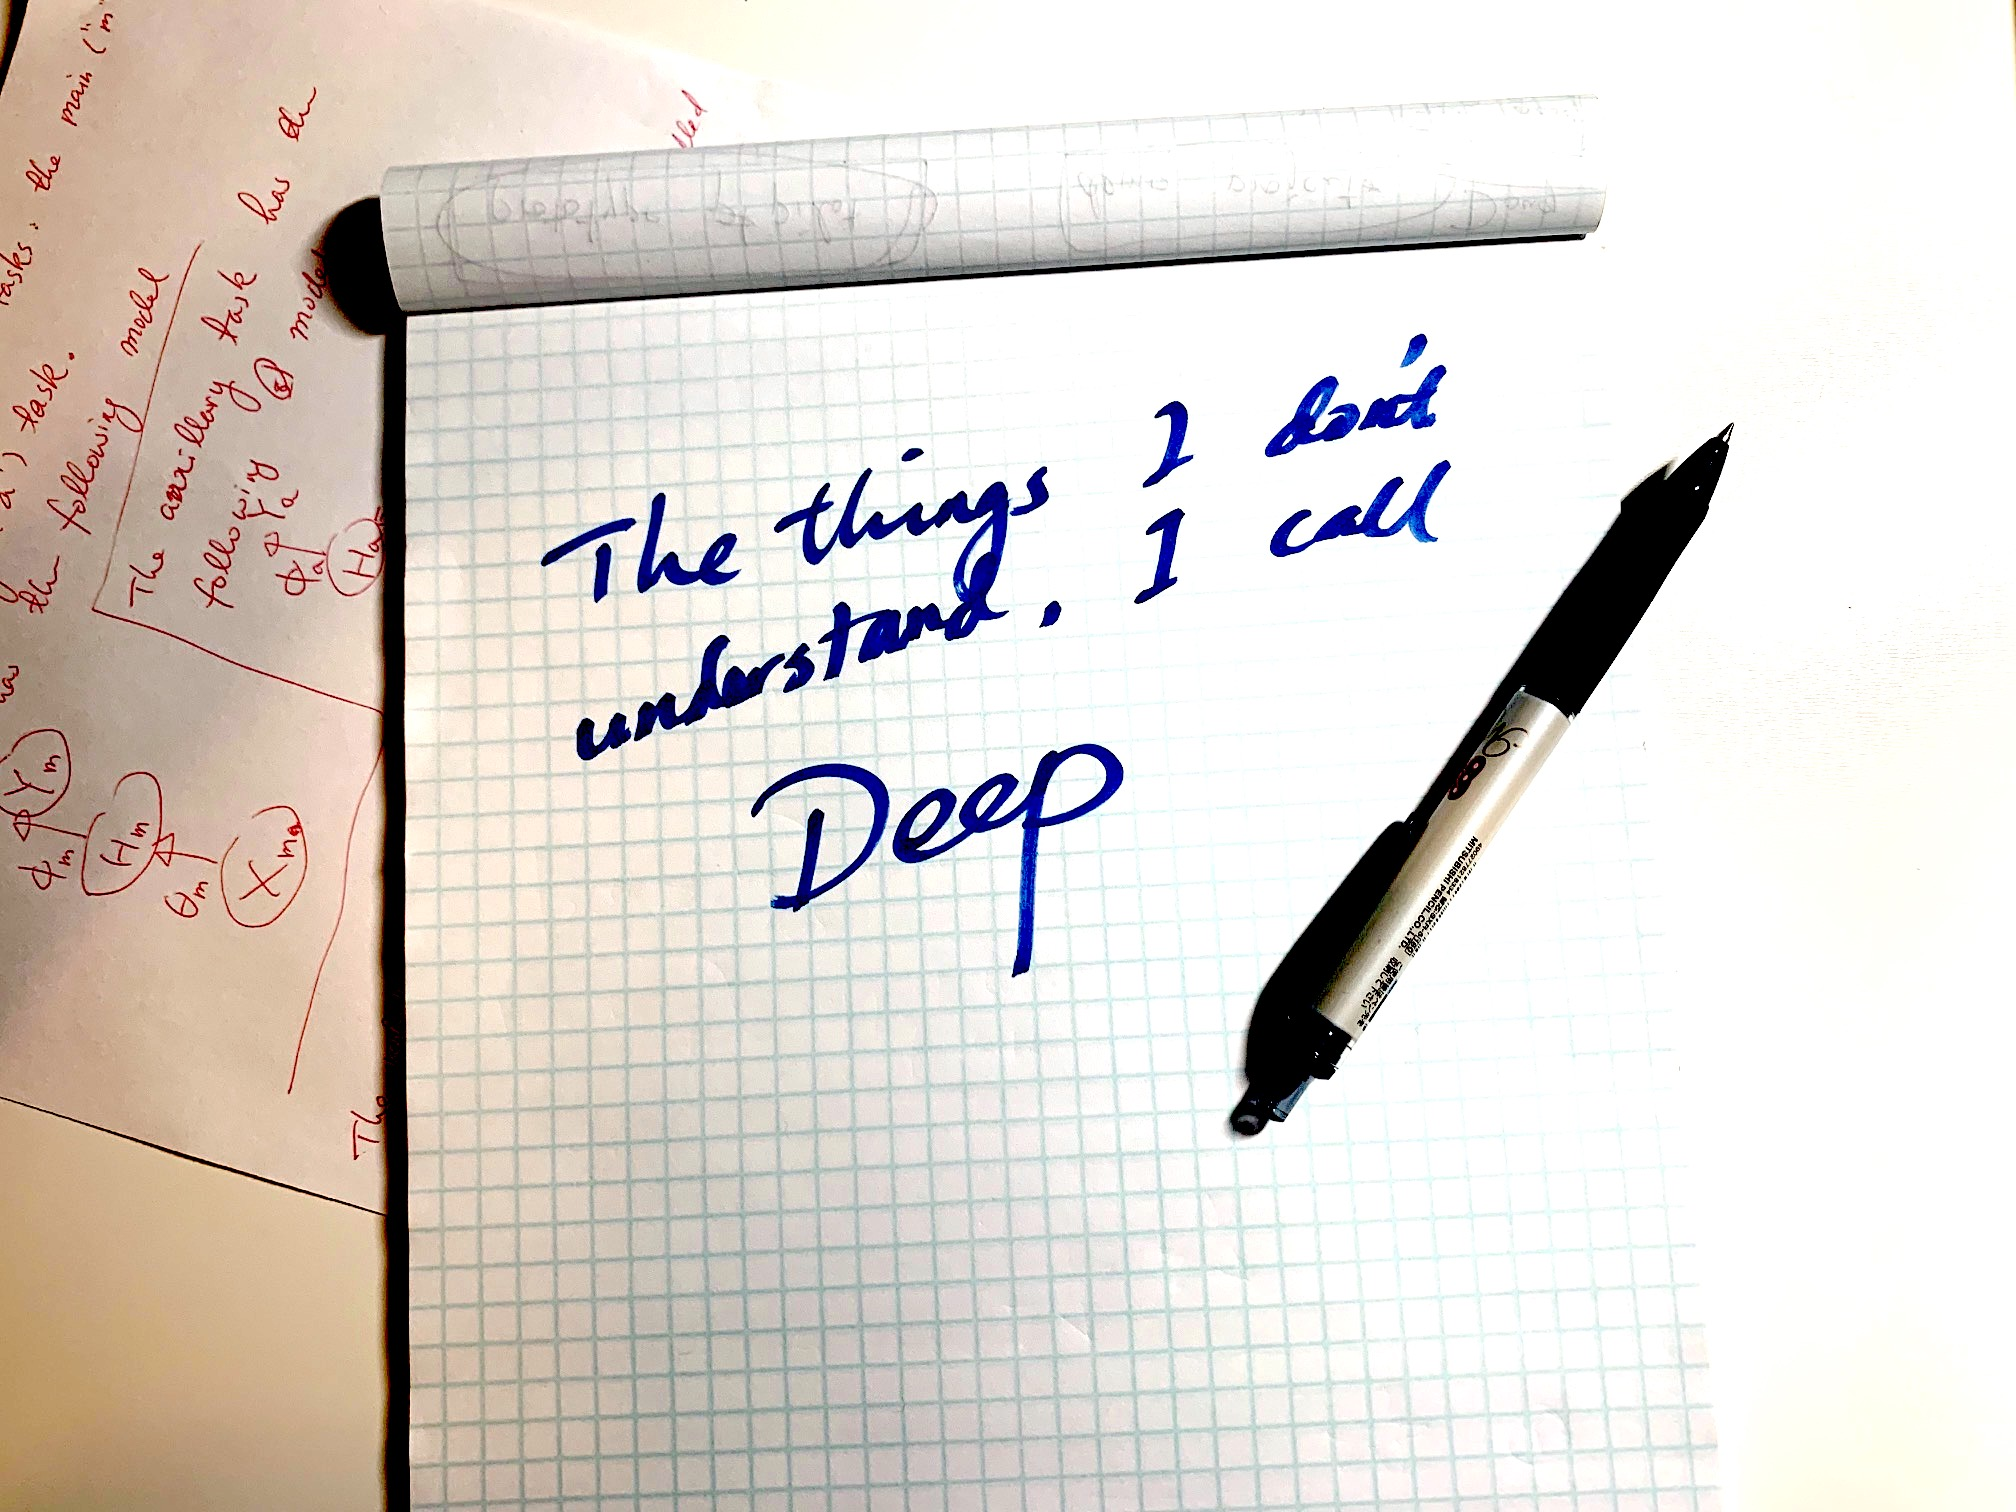
\includegraphics{testImage.jpg}}
\caption{The logo of the course}
\label{fig:logo}
\end{figure}


\section{Syllabus}

We will use a strange way to grade. 

\[
y=x_0\cdot x_1 + x_2 + x_3
\]


\section{Math}
Consider the following example.
\begin{ex}
Suppose that $p_X$ is the Bernoulli distribution defined as in the
previous example and that random variable $Y$ is defined by
\[
Y=p_X(X).
\]
Find the PMF of $Y$.
\end{ex}

\noindent{Answer:}

First we identify $p_X$ as a function mapping $\Omega_X:=\{0, 1\}$
into $\Omega_Y:={\mathbb R}$.  

If $\mu=0.5$, then
\[
p_Y(y)=\left\{
\begin{array}{ll}
1,& {\rm if}~y=0.5,\\
0, & {\rm otherwise}.
\end{array}
\right.
\]
That is, $Y$ is deterministically $0.5$.
If $\mu \neq 0.5$, then
\[
p_Y(y)=\left\{
\begin{array}{ll}
\mu,& {\rm if}~y=\mu,\\
1-\mu, & {\rm if}~y=1-\mu,\\
0, &{\rm otherwise}.
\end{array}
\right.
\]



\section*{Appendix: \LaTeX ing Your Lecture Script}

 Some extra commands are provided by the 
{\tt scribe} package, which may  not be used in the above notes.  
You may open the {\tt scribe.sty} file 
to see this if you have known quite a bit about \LaTeX; alternatively, 
you may open the \LaTeX\ source file of 
this document to see how the following formatted text is generated. 


\begin{definition}
A software is said to be {\em OK} if it is free. 
\end{definition}

\begin{definition}
An OK  software is said to be {\em good} if it is bug-free.
\end{definition}

\begin{definition}
A good software is said to be {\em excellent} if it provides
user-desired functionalities.
\end{definition}



\begin{lemma}
Microsoft WORD is not OK.
\end{lemma}

\Proof :\\
This follows immediately from the definition of OK.
\QED

\begin{lemma}
\LaTeX\ is OK.
\end{lemma}

\Proof :\\
This follows immediately from the definition of ``OK''.
\QED

\begin{proposition}
\LaTeX\ is good.
\end{proposition}

\Proof :\\
This follows immediately from the definition of ``good''.
\QED

\begin{theorem} \LaTeX\ is excellent.
\end{theorem}

\Proof :\\
This follows immediately from the definition of ``excellent''.
\QED

\begin{corollary}
\LaTeX\  is better than Microsoft WORD, with the metric of goodness
defined as above.
\end{corollary}

\Proof :\\
This is a consequence of the first lemma and the above theorem. \QED

\begin{hw}
Remove WINDOWS from your PC, and install Linux. 
\LaTeX\ is there.
\end{hw}

\begin{hw}
Learn \LaTeX.
\end{hw}



\end{lecture}

\end{document}
